	\newpage
\section{Projektowanie}		%3
%Napisać z jakich narzędzi będziemy korzystać (kompilator, język programowania), git, biblioteki dodatkowe, itp.
%Opisać szczegółowe ustawienia kompilatora (jeśli są), powiązania z bibliotekami, itp.
%Narysować graf, UML, diagram klas, schemat działania algorytmu
\hspace{0.60cm}Projekt wykonany będzie w programie Virtual Studio Code z użyciem języka C++. Kompilacja będzie przeprowadzana za pomocą dodatku do VS Code o nazwie Code Runner wykorzystującego wcześniej zainstalowany kompilator MinGW. Kolejne wersje projektu będą zapisywane na platformie GitHub.

\begin{figure}[!htb]
	\begin{center}
		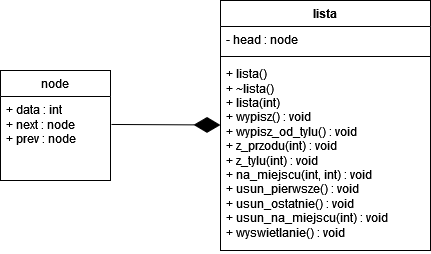
\includegraphics{Dokumentacja/rys/UML.png}
		\caption{Diagram klasy.}
		\label{rys:rysunek009}
	\end{center}
\end{figure}

\hspace{0.60cm}Klasa będzie zawierać strukturę node odpowiadającą poszczególnym elementom listy. Działanie wszystkich metod klasy będzie przetestowane w funkcji main.